

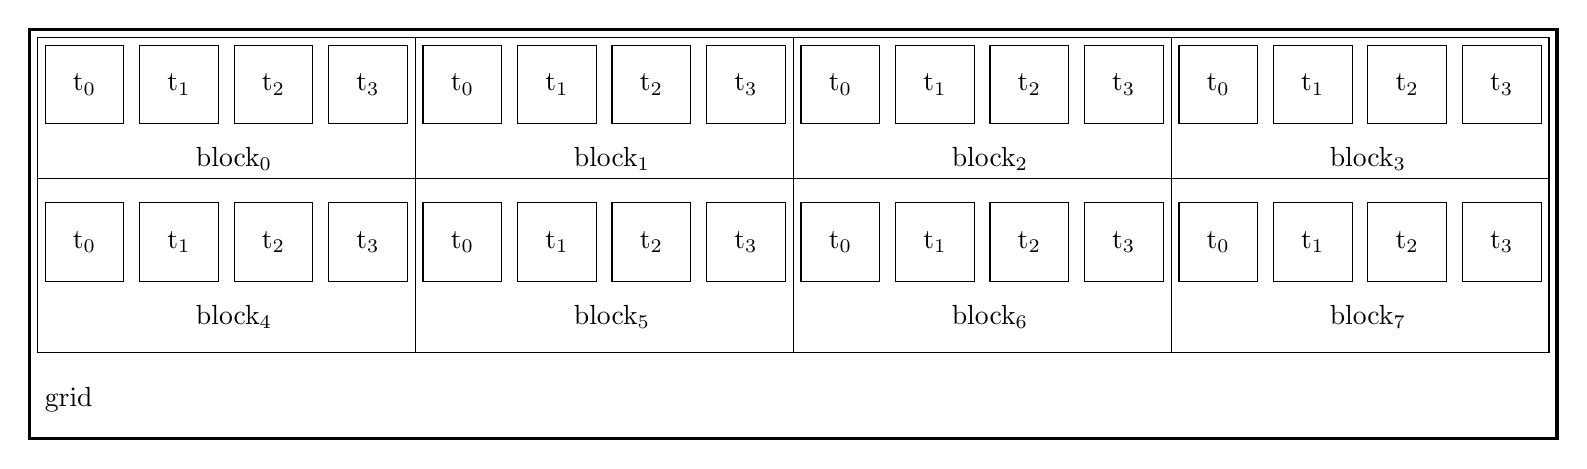
\begin{tikzpicture}[]


    %%% DEFINITIONS %%%%%%%%%%%%%%%%%%%%%%%%%%%%%%%%%%%%%%%%%%%%%%%%%%%%%%%%%%%%%
    
    
    % https://associatie.kuleuven.be/huisstijl/kleuren
    \definecolor{blue1}{RGB}{82,189,236}
    \definecolor{blue2}{RGB}{0,64,122}
    \definecolor{blue3}{RGB}{31,171,231}
    \definecolor{blue4}{RGB}{29,141,176}
    \definecolor{blue5}{RGB}{17,110,138}
    \definecolor{orange1}{RGB}{221,138,46}
    
    
    \def\SignalY{2}
    \def\GridOneY{-3.5}
    \def\GridTwoY{0}
    \def\MultiplierX{1.2}
    
    \def\SquareSize{1}
    
    \def\ThPoolCenterTwoX{2}
    \def\ThPoolCenterTwoY{0}
    
    \def\NumOfSamples{16}
    
    \def\BlockDimX{4}
    
    
    %%% DRAWING %%%%%%%%%%%%%%%%%%%%%%%%%%%%%%%%%%%%%%%%%%%%%%%%%%%%%%%%%%%%%%%%%
    
    
    
    \foreach \b in {0,...,3} {
        \foreach \t in {0,...,3} {
            \pgfmathsetmacro{\res}{int(\t+\BlockDimX*\b)}
            \draw[black] ({(\t + \b * \BlockDimX) * \MultiplierX}, \GridOneY) rectangle ++ (\SquareSize, \SquareSize);
            \node at ({(\t + \SquareSize * \b * \BlockDimX) * \MultiplierX + \SquareSize/2}, \GridOneY + \SquareSize/2) {t$_{\t}$};
        }
        \draw[black] (-0.1 + \b * \MultiplierX * \BlockDimX, \GridOneY - 0.1 - 0.6) rectangle ++ (\SquareSize * \MultiplierX * \BlockDimX, \SquareSize + 0.2 + 0.6);
        \node at ({(\b + 0.5) * \MultiplierX * \BlockDimX}, \GridOneY - 0.45) {block$_\b$};
    }

    \foreach \b in {0,...,3} {
        \foreach \t in {0,...,3} {
            \pgfmathsetmacro{\res}{int(\t+\BlockDimX*\b)}
            \draw[black] ({(\t + \b * \BlockDimX) * \MultiplierX}, \GridOneY - 2) rectangle ++ (\SquareSize, \SquareSize);
            \node at ({(\t + \SquareSize * \b * \BlockDimX) * \MultiplierX + \SquareSize/2}, \GridOneY + \SquareSize/2 - 2) {t$_{\t}$};
        }
        \draw[black] (-0.1 + \b * \MultiplierX * \BlockDimX, \GridOneY - 0.1 - 0.6) rectangle ++ (\SquareSize * \MultiplierX * \BlockDimX, \SquareSize + 0.2 + 0.6 - 4);
        \node at ({(\b + 0.5) * \MultiplierX * \BlockDimX}, \GridOneY - 0.45 - 2) {block$_{\the\numexpr\b+4}$};
    }
    
    
    \draw[black, very thick] (-0.2, \GridOneY - 0.2 - 0.6 - 0.6 - 2.6) rectangle ++ (\SquareSize * \MultiplierX * \NumOfSamples + 0.2, 2* \SquareSize + 3.2 );
    \node at (0.3, \GridOneY-3.5) {grid};
    
    %\node[rotate=90] at (-0.75, \GridOneY) {[3, 4]};
    %\node[rotate=90] at (\SquareSize * \MultiplierX * \NumOfSamples + 0.5, \GridOneY) {[3, 4]};
    
    
    
    

    
    
    
    \end{tikzpicture}